\documentclass[letterpaper, 10 pt, conference]{ieeeconf}  % Comment this line out if you need a4paper
%\documentclass[a4paper, 10pt, conference]{ieeeconf}   % Use this line for a4 paper
\IEEEoverridecommandlockouts                                    % This command is only needed if you want to use the \thanks command
\overrideIEEEmargins                                                 % Needed to meet printer requirements.

%In case you encounter the following error:
%Error 1010 The PDF file may be corrupt (unable to open PDF file) OR
%Error 1000 An error occurred while parsing a contents stream. Unable to analyze the PDF file.
%This is a known problem with pdfLaTeX conversion filter. The file cannot be opened with acrobat reader
%Please use one of the alternatives below to circumvent this error by uncommenting one or the other
%\pdfobjcompresslevel=0
%\pdfminorversion=4

% See the \addtolength command later in the file to balance the column lengths
% on the last page of the document

\usepackage{graphicx}    % for pdf, bitmapped graphics files
%\usepackage{epsfig}    % for postscript graphics files
\usepackage{mathptmx} % assumes new font selection scheme installed
\usepackage{times}        % assumes new font selection scheme installed
\usepackage{amsmath}  % assumes amsmath package installed
\usepackage{amssymb}  % assumes amsmath package installed
\usepackage{multirow}    % for aligning table column headers that span columns

\title{\LARGE \bf Multi-robot Formation Control}

\author{Ajay Ahir, Ben Philps and Sumaiyah Kola}

\begin{document}

\maketitle
\thispagestyle{empty}
\pagestyle{empty}

%%%%%%%%%%%%%%%%%%%%%%%%%%%%%%%%%%%%%%%%%%%%%%%%%%%%%%%%%%%%%%%%%%%%%%%%%%%%%%%%
\begin{abstract}
	
Multi-robot formations have proved useful in applications for exploration, surveillance and `search and rescue'. In such domains reliable global communication is not a guarantee. In this paper we implement a centralized and decentralized approach to multi-robot formation control that includes a reactive formation switching strategy. The robot formations successfully navigate through obstacle fields, tight corners and narrow corridors.

\end{abstract}
	
%%%%%%%%%%%%%%%%%%%%%%%%%%%%%%%%%%%%%%%%%%%%%%%%%%%%%%%%%%%%%%%%%%%%%%%%%%%%%%%%
\section{INTRODUCTION}
	
In application domains such as exploration, surveillance and `search and rescue', coordination and control mechanisms for multiple robots have been shown to provide cost effective and fault tolerant solutions \cite{c1}.

Inspired by the natural coordinated behavior of bird flocking and ant swarming, formation control of multiple robots can improve surveillance coverage by combining sensor readings from individual agents. The main objective is for multiple robots to traverse the environment while maintaining an explicitly specified spacing relationship between agents.

In this paper we provide a centralized behavior-based approach to formation control. This solution relies on each agent transmitting and receiving information from a global controller. We also provide a robust and fault-tolerant decentralized approach suitable when communication is restricted.

\subsection{BACKGROUND}
\label{background}

Balch and Arkin provide a behavior-based approach to formation control, splitting the task into behavioral components, referred to as `motor schemas' \cite{c2}. 

\subsubsection*{Motor Schemas}

Given the current sensor inputs and robot positions, each motor schema generates a behavioral response as a vector $\vec{V}_s$ with a direction and magnitude of desired movement. Motor schemas goal navigation, static/dynamic obstacle avoidance and formation maintenance generate vectors $\vec{V}_{goal}, \vec{V}_{static\_obs}, \vec{V}_{dynamic\_obs}, \vec{V}_{form}$ respectively. A gain value $g_s$ dictates the contribution of each schema to the overall behavior.  

The overall behavioral response $\vec{V}$ is calculated by weighting each vector by its gain value then summing and normalizing the result. To overcome minima an additional schema generating noise $\vec{V}_{noise}$ is included.

\subsubsection*{Formation Maintenance}

To compute $\vec{V}_{form}$ for robot $R_i$ in position $P_{R_i}$,
\[\vec{V}_{form} = P_{desired} - P_{R_i}\]
where $P_{desired}$ is the desired position of $R_i$ in the formation. 
Unit-, leader- and neighbor-referenced techniques exist to determine the formation position $P_{desired}$.

The magnitude of $\vec{V}_{form}$ depends on the distance between $P_{R_i}$ and $P_{desired}$. `Zones' are defined around $P_{desired}$ as seen in Fig. \ref{formation_zones}. 

Within the \textit{dead zone}, the robot is considered in formation and so $\vec{V}_{form} = \vec{0}$. Within the \textit{control zone}, the magnitude linearly increases from the inner edge. The magnitude at the outer edge of the \textit{control zone} is propagated throughout the \textit{ballistic zone}.

\begin{figure}[ht]
\centering
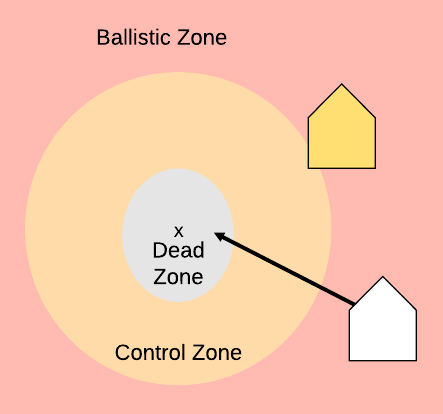
\includegraphics[width=0.45\linewidth]{images/formation_zones.png}
\caption{Zones for computing $\vec{V}_{form}$ with $P_{desired}$ marked as `x'}
\label{formation_zones}
\end{figure}

We implement a leader-referenced behavior-based approach to formation control, extending the work of Balch and Arkin to incorporate a formation switching strategy.

\section{APPROACH}

We implement a centralized and decentralized leader-referenced approach to formation control. 

A leader-referenced approach is chosen as each robot need only know the position of the leader $R_0$ to determine its own position in the formation. In contrast, for a unit-referenced approach each robot needs the positions of all other robots in the formation. This would require the transmission of more state.

Motor schemas for goal navigation, static obstacle avoidance and formation maintenance are defined. Vectors from each motor schema are combined into an overall behavioral response $\vec{V}$ for each robot.

Dynamic obstacle avoidance applies to the other robots. We produce a weight vector $W$ which takes value $0$ to tell robot $R_i$ to stop moving if it is behind robot $R_j$, and is $1$ otherwise. If the two robots are approximately adjacent then the robot with the lowest ID stops and the other moves to avoid deadlock. The weight is computed based on the distance between robots and how much they face each other.

We use feedback linearization to convert the behavioral response $\vec{V}$ into control inputs $\mu$ and $\omega$, corresponding to linear and angular velocity respectively. Feedback linearization assumes the robot is held by a holonomic point at a distance of $\epsilon$. Here $\epsilon$ is 0.2m.

\subsection{EXPERIMENTAL SET-UP}

We conduct experiments on TurtleBot3 \cite{turtlebot} robots controlled using ROS \cite{ros} with Gazebo \cite{gazebo} as the simulation environment. We assume all robots are identical and labeled, with $R_0$ designated as leader and $R_1,...,R_n$ as followers. Here $n$ is 4.

Our evaluation considers the performance of robot formations in multiple arenas that include obstacles, narrow corridors and tight corners. Fig. \ref{corridorworld} illustrates one of the testing arenas.

\begin{figure}[thpb]
\centering
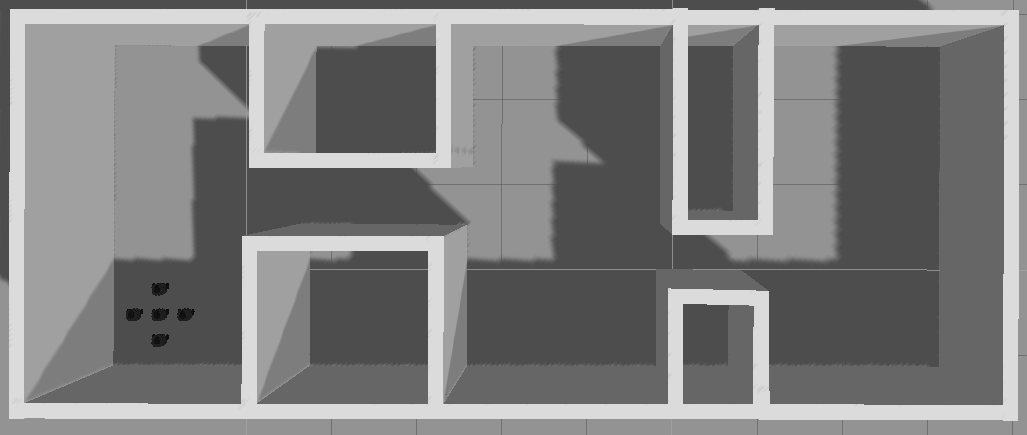
\includegraphics[width=\linewidth]{images/corridorworld.png}
\caption{The \textit{diamond} formation in an arena with tight corridors}
\label{corridorworld}
\end{figure}

\subsection{FORMATIONS}

In our implementation \cite{repository}, four formations for five robots are considered: \textit{diamond}, \textit{column}, \textit{line} and \textit{wedge} (Fig. \ref{formation_shapes}). Each formation is defined as a vector of coordinates relative to the leader. The spacing of the robots in the formation can be altered. 

\begin{figure}[thpb]
\centering
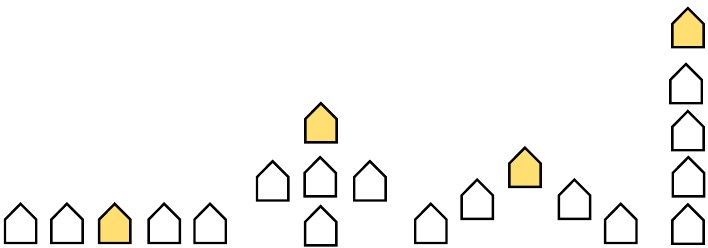
\includegraphics[width=0.7\linewidth]{images/formation_shapes.jpg}
\caption{Formations L-R: \textit{line}, \textit{diamond}, \textit{wedge}, \textit{column} with leader colored}
\label{formation_shapes}
\end{figure}

\subsection{MOTOR SCHEMAS}

In our approach, the objective of the leader is to reach the goal while avoiding obstacles and other robots. The leader does not attempt to maintain formation. Only follower robots $R_1,...,R_n$ are responsible for formation maintenance. 

Consequently, the behavioral response $\vec{V}$ for each robot is,
\begin{equation*}
\begin{aligned}
\vec{V} = & g_{goal} \vec{V}_{goal} + g_{obs} \vec{V}_{obs} + \vec{V}_{noise}    && \text{if leader} \\
              & g_{form} \vec{V}_{form} + g_{obs} \vec{V}_{obs} + \vec{V}_{noise}   && \text{if follower} \\
\end{aligned}
\end{equation*}
where $\vec{V}_{noise}$ has a magnitude of 0.05. Table \ref{motor_schema_gs} contains the gain values for each motor schema. The values were tuned empirically to allow the formation to split around an obstacle and merge when possible.

\begin{table}[h]
\begin{center}
\begin{tabular}{|c|c|c c|}
\hline
Motor Schema & Gain Value \\
\hline
Goal Navigation                  & 0.35 \\
Static Obstacle Avoidance    & 0.22 \\
Formation Maintenance       & 0.20 \\
\hline
\end{tabular}
\end{center}
\caption{Motor Schema Gain Values $g_s$}
\label{motor_schema_gs}
\end{table}

\subsubsection*{Goal Navigation}

$\vec{V}_{goal}$ points from the leader $R_0$ to the next point along a path from $P_{R_0}$ to the goal. A path is generated using an optimized version of the rapidly-exploring random trees (RRT) algorithm, RRT*. RRT efficiently explores the search space by building a space-filling tree. Additional rewiring and cost minimization steps can generate an approximate shortest path to the goal. The magnitude of $\vec{V}_{goal}$ is 1.

\subsubsection*{Static Obstacle Avoidance}

We implemented a hybrid braitenberg/rule-based controller to avoid obstacles such as walls. The addition of rules dictates the direction a robot should turn based on which side of the formation it lies on, and the resulting vector is scaled to have maximum magnitude $1$.

\subsubsection*{Formation Maintenance}

We use the implementation of this motor schema defined in Balch and Arkin and described in \ref{background}. Only the follower robots need to compute $V_{form}$ as the leader is considered to always be in formation.

To calculate $P_{desired}$ we transform the vector of relative formation positions, by rotating it to match the leader's orientation then translating it to the leader's position.

We normalize $V_{form}$ by computing $V_{form}/|control\_zone|$. Table \ref{table_formation} contains the parameters we used to implement this motor schema.

\begin{table}[h]
\begin{center}
\begin{tabular}{|c|c|c|}
\hline
& Parameter & Value (m) \\
\hline
(1) & Robot Radius             & 0.05 \\
(2) & Spacing Distance        & 0.8 \\
(3) & Dead Zone Radius      & $1.5 \times (1) = 0.075$ \\
(4) & Control Zone Radius    & (2) $+$ (3) $=0.875$ \\
\hline
\end{tabular}
\end{center}
\caption{Formation Maintenance Parameters}
\label{table_formation}
\end{table}

\subsection{FORMATION SWITCHING STRATEGY}

We implement a reactive formation switching strategy to determine the safest formation, given the current environment. A robot is said to `detect' a corridor if the \textit{left} and \textit{right} sensors report measurements less than a threshold, here 0.4m, and the environment ahead of the \textit{front} sensor is clear.

If the leader or at least half of the followers detect a corridor, the formation is switched to a \textit{column} until robots exit the corridor and it is safe to return to the default formation. We chose \textit{column} as it is the narrowest formation.

\subsection{DECENTRALIZED}

The centralized algorithm relies on knowledge of all robot positions as well as their combined view of the world. Our decentralized solution achieves this with limited message passing between robots to communicate the required state. Communication links are defined between certain robots in each formation. For \textit{line}, \textit{column} and \textit{wedge}, links are defined between adjacent robots. For \textit{diamond}, all robots are arranged so they can communicate with the center robot.

Our consensus algorithm uses each robot's ID to decide the leader. Robot $R_i$ is the leader if,
\[\text{form\_pos}[ID(R_i)] = (0,0)\]
Where `form\_pos' is the vector of relative formation positions and `$ID$' returns a robot's ID. IDs are assigned in such a way that each corresponds to a unique position. Only the leader initiates message passing when their state updates, and the other robots relay this message down their formation links, excluding the receiving link.

Decentralized obstacle avoidance is slightly different to centralized obstacle avoidance. The braitenberg hybrid controller uses the additional knowledge of every other robot to compute which side of the formation a robot is on. As we do not have this state in the decentralized approach, we only use a rule-based controller.

\section{RESULTS}

We evaluate the performance of the centralized and decentralized approach in the

TODO:NAME arena.

TODO: write this up properly

1: Centralized algorithm

2: Decentralized algorithm
	
\begin{table}[h]
\begin{center}
\begin{tabular}{|c c|c|}
\hline
\multicolumn{2}{|c|}{Formation} & Error \\
Default & Safety & \\
\hline
\textit{diamond}    & \textit{column} & 0 \\
\textit{wedge}       & \textit{column} & 0 \\
\textit{line}           & \textit{column} & 0 \\
\hline
\end{tabular}
\end{center}
\caption{Pose Error in Centralized algorithm}
\label{table_results_centralized}
\end{table}

\begin{table}[h]
\begin{center}
\begin{tabular}{|c c|c|}
\hline
\multicolumn{2}{|c|}{Formation} & Error \\
Default & Safety & \\
\hline
\textit{diamond}    & \textit{column} & 0 \\
\textit{wedge}       & \textit{column} & 0 \\
\textit{line}           & \textit{column} & 0 \\
\hline
\end{tabular}
\end{center}
\caption{Pose Error in Decentralized algorithm}
\label{table_results_decentralized}
\end{table}

\section{CONCLUSION}

\addtolength{\textheight}{-12cm}   % This command serves to balance the column lengths
                                               % on the last page of the document manually. It shortens
                                               % the textheight of the last page by a suitable amount.
                                               % This command does not take effect until the next page
                                               % so it should come on the page before the last. Make
                                               % sure that you do not shorten the textheight too much.

%%%%%%%%%%%%%%%%%%%%%%%%%%%%%%%%%%%%%%%%%%%%%%%%%%%%%%%%%%%%%%%%%%%%%%%%%%%%%%%%
\section{ACKNOWLEDGMENT}

\begin{itemize}
\item Ajay Ahir - Worked on setting up the multi-robot environment and obstacle avoidance. Added the RRT* component and worked on combining velocities. Decentralized the solution and produced the error plots.

\item Ben Philps - 

\item Sumaiyah Kola - 
\end{itemize}

%%%%%%%%%%%%%%%%%%%%%%%%%%%%%%%%%%%%%%%%%%%%%%%%%%%%%%%%%%%%%%%%%%%%%%%%%%%%%%%%
\begin{thebibliography}{99}
	
\bibitem{c1} J. S. Jennings, G. Whelan and W. F. Evans, ``Cooperative Search and Rescue with a Team of Mobile Robots'', 8th International Conference on Advanced Robotics, Proceedings ICAR'97, Monterey, CA, USA, pp. 193-200, Jul. 1997.

\bibitem{c2} T. Balch and R. C. Arkin, ``Behavior-based Formation Control for Multi-robot Teams'', IEEE Transactions on Robotics and Automation, vol. 14, no. 6, pp. 926-939, Dec. 1998.

\bibitem{turtlebot} TurtleBot3, http://emanual.robotis.com/docs/en/platform/turtlebot3/overview/
\bibitem{ros} ROS - Robot Operating System, https://www.ros.org/
\bibitem{gazebo} Gazebo, http://gazebosim.org/
\bibitem{repository} Code Repository, https://github.com/DoodleBobBuffPants/RobotProject

\end{thebibliography}

\end{document}

